\documentclass[11pt,		% 11pt Schrift
	    %BCOR8mm, 		% Bindekorrektur
	    DIV12,		% Satzspiegel
	    %twoside,		% Doppelseitige Ausgabe
	    a4paper,		% DIN A4
	    %openright,		% Neue Kapitel auf rechter Seite
%	    dvips,		% Source Specials ins DVI/PS	
%	    draft,		% Bilder weglassen, Overfull H-Boxen markieren
	    final,		% Engültige Version mit Bildern
	    %cleardoubleplain,	% leere linke Seite bei openright
	    halfparskip,	% Absatzabstand
	    ]{scrartcl}		% KOMA-Skript Klasse


% Kodierung des Quelltextes
\usepackage[english]{babel}
%\usepackage[latin1]{inputenc} % Latin1
\usepackage[utf8]{inputenc} 	% UTF-8
% Kodierungskram im Zieldokument
\usepackage[T1]{fontenc}
%\KOMAoptions{pagesize=dvips}


%%% OPTIK %%%%%%%%%%%%%%%%%%%%%%%%%%%%%%%%%%%%%%%%%%%%%%%%%%%%%%%%%%%%%%%%%%
% Schriftart Palatino
% -> 11pt einstellen
\usepackage{mathpazo} 	% Schriftart Palatino
\linespread{1.1}	% Zeilenabstand

\typearea[current]{last} % Satzspiegel für Schriftart erneut berechnen

% Ueberschriften fett
\setkomafont{sectioning}{\normalcolor\bfseries}
% Bild- und Tabellen-Unterschriften formatieren
\renewcommand{\caplabelfont}{\bfseries}
\renewcommand{\capfont}{\small}

% fuer subfigure
\newcommand{\goodgap}{%
\hspace{\subfigtopskip}%
\hspace{\subfigbottomskip}}


%%% PACKAGES %%%%%%%%%%%%%%%%%%%%%%%%%%%%%%%%%%%%%%%%%%%%%%%%%%%%%%%%%%%%%%%%%
% Paket zum Einbinden von Grafiken
% final: Grafiken auch bei draft einbinden
\usepackage[final]{graphicx}

% Automatische Hyperlinks bei Referenzen/Verweisen (verschwinden beim Druck)
\usepackage[final=true, breaklinks=true]{hyperref}

% Literaturverzeichnis nach deutscher Norm
%\usepackage{bibgerm}

% Lange Tabellen (mehr als eine Seite) 
%\usepackage{longtable}

% AMS-Math Paket
\usepackage{amsmath,amssymb}

% Grafiken mit LaTeX beschriften
\usepackage{psfrag}
% Abbildungen mit Unterabbildungen
%\usepackage{subfigure}
\usepackage{longtable}
\usepackage{caption}
\usepackage{subcaption}
% Schoene Darstellung physikalischer Einheiten
\usepackage{nicefrac}
\usepackage{units}

%%% DOCUMENT %%%%%%%%%%%%%%%%%%%%%%%%%%%%%%%%%%%%%%%%%%%%%%%%%%%%%%%%%%%%%%%%%
\begin{document}
\begin{center}
{\huge GSoC 2014: Increasing the throughput of the GR-Trellis module and adding an OOT Turbo Equalizer Module}\\[1cm]
{Jan Krämer}\\[0.25cm]
{kraemer@int.uni-karlsruhe.de}\\[0.5cm]
{12.03.2014}\\[0.5cm]
\end{center}
\tableofcontents 
\newpage
\section{Introduction}
Trellis-based error-coding is a powerful tool to deal with corrupted data in high bandwidth mobile communication systems. The data in mobile communication systems is often encoded with a convolutional code at the transmitter. This enables the receiver to correct errors that are induced by the channel. Usually, this is done by a Viterbi algorithm or a Maximum A Posteriori (MAP) algorithm (e.g. BCJR). Both approaches are complex and hence determine the data throughput at the receiver. To design efficient implementations in software is an important topic in the context of software defined radio. The bit error rate (BER) performance can be further improved by using concatenated convolutional codes. This principle is called turbo code. Turbo codes require a special decoder structure composed of two separate decoders that iteratively exchange soft information about the codebits \cite{tc02}. If communication is performed over a multipath channel that induces intersymbol interference (ISI), it can be interpreted as a second convolutional code. The resulting decoder structure is similar to a turbo decoder but the outer decoder is swapped for an equalizer. This structure is called turbo equalizer \cite{te02}. To reduce the receiver complexity, the equalizer is often implemented as a linear Minimum Mean Square Error (MMSE) equalizer. An overview over these three approaches (single convolution code, turbo code, turbo equalizer) is given in figures \ref{fig:dec}-\ref{fig:turboeq}.\\ \\ The goal of this project is to improve the data throughput of the gr-trellis module, as suggested by Achilleas Anastasopoulos\footnote[1]{http://lists.gnu.org/archive/html/discuss-gnuradio/2014-02/msg00444.html} and Tom Rondeau\footnote[2]{http://lists.gnu.org/archive/html/discuss-gnuradio/2014-02/msg00445.html} on the GNURadio mailinglist. This is crucial for developing waveforms for high bandwidth mobile communication systems. As the gr-trellis module is also the basis for future turbo decoder/equalizer modules in GNURadio, gr-trellis has to be implemented as efficient as possible before starting to implement structures that apply the turbo principle. This can be done by improving the single thread performance with SIMD instructions and by adding multiprocessor support and exploiting parallel structures in the decoder algorithm.\\ \\Some theoretical basics on trellis-based decoding are given in chapter two. Chapter three includes deliverables and chapter four introduces a preliminary timetable for this project. A final conclusion is given in chapter five. At the end, I would like to illustrate my motivation to participate in GSoC 2014 and why I chose this project.  
\begin{figure}[htbp] 
  \centering
  \begin{subfigure}[bt]{0.45\textwidth}
       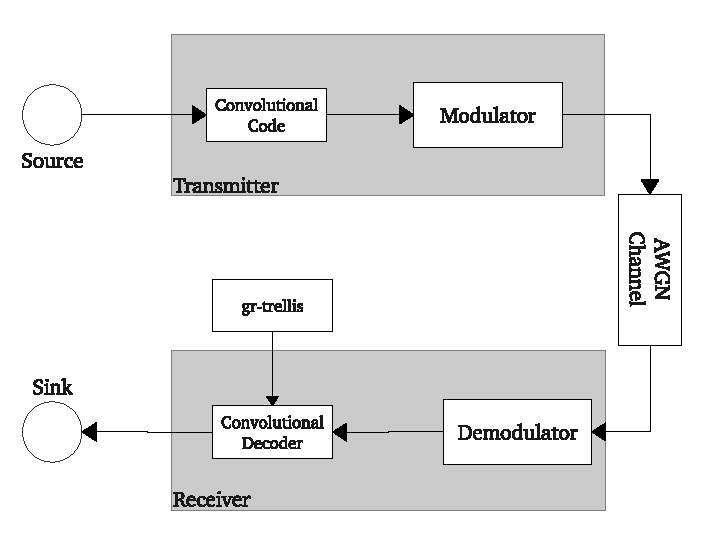
\includegraphics[width=0.8\textwidth]{figures/dec.eps}
  \caption{Convolutional code/AWGN channel}
    \label{fig:dec}
  \end{subfigure}
  \begin{subfigure}[bt] {0.45\textwidth}
     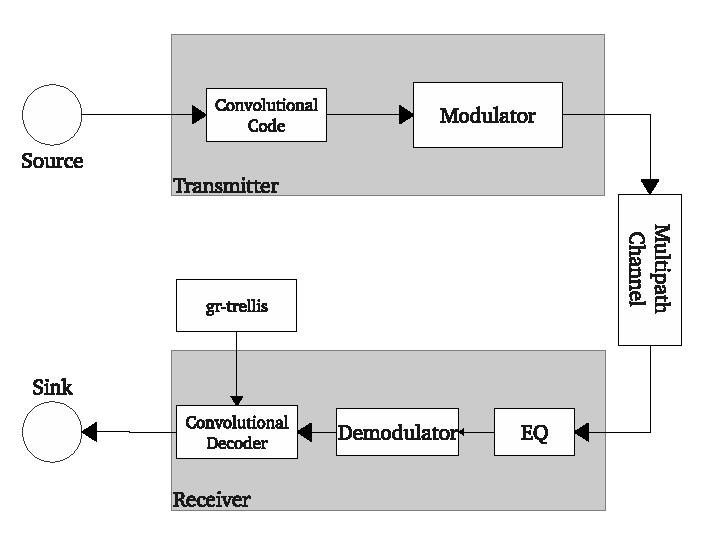
\includegraphics[width=0.8\textwidth]{figures/deceq.eps}
  \caption{Convolutional code/multipath channel}
    \label{fig:eq}
  \end{subfigure}
  \begin{subfigure}[bt]{0.45\textwidth}
       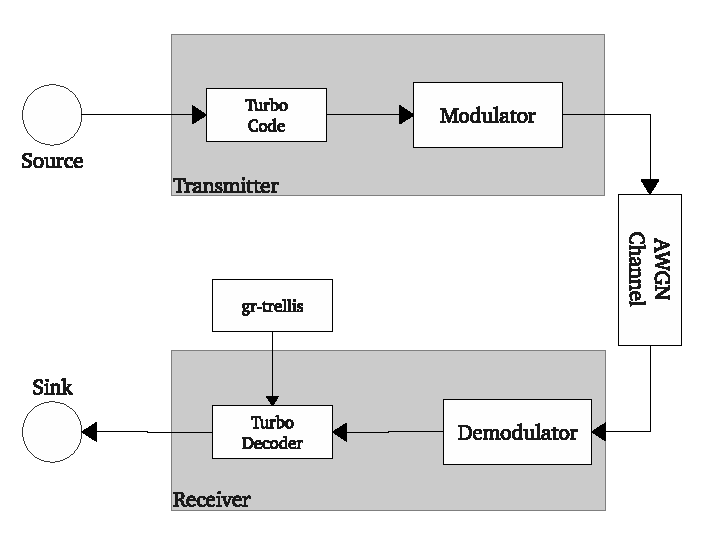
\includegraphics[width=0.8\textwidth]{figures/turbodec.eps}
  \caption{Turbo Decoder}
    \label{fig:turbodec}
  \end{subfigure}
  \begin{subfigure}[bt] {0.45\textwidth}
     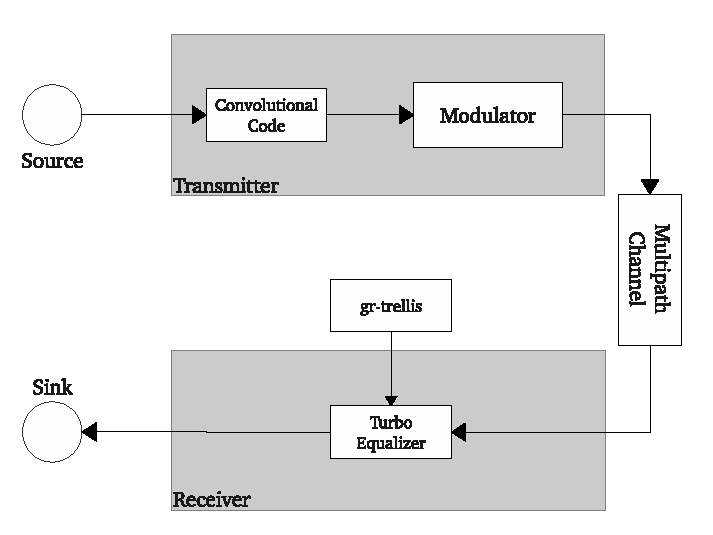
\includegraphics[width=0.8\textwidth]{figures/turboeq.eps}
  \caption{Turbo EQ}
    \label{fig:turboeq}
  \end{subfigure}  
  \caption{AWGN and multipath communication scenarios}
    
\end{figure}
\section{Trellis-based Decoding}
The theory behind trellis-based decoding is complex. Therefore I will only present a short summary of the main ideas behind this approach. To use trellis-based algorithms, like Viterbi or BCJR algorithm, the data has to be encoded by the transmitter. In mobile communication systems, this is usually done with a convolutional encoder. Convolutional encoders can be interpreted as a finite state machine. Their output depends on the current state and the input data. This structure constrains the output signal and adds redundancy which then can be used to correct corrupted data in the receiver. \\ \\In the gr-trellis module, this is done through either a Viterbi or a Soft Input Soft Output (SISO) algorithm \cite{gnrDoc}. The Viterbi algorithm is a sequence decoder as it calculates the most probable path through the trellis by using a Maximum Likelihood (ML) algorithm. The SISO algorithm operates on the entire received sequence and finds the most probable codebit by calculating the probabilities for every possible produced codebit or databit. The SISO algorithm uses a Maximum A Posteriori (MAP) algorithm. Both are computational heavy algorithms and unoptimized implementations will result in low data rates as already mentioned in section $1$. 
\section{Deliverables}
\begin{description}
  \item[Improving single thread performance:] Single thread performance can be increased by using VOLK. This will make use of SIMD systems and improve the speed of those calculations that can exploit data level parallelism. Possible targets are:
  \begin{itemize}
        \item Metric calculations in calc\_metric.cc. Euclidean metrics can be calculated for several output symbols or several time steps in parallel. 
        \item Update metrics for several states in parallel in core\_algorithms.cc.  
        \item Metric normalization in core\_algorithms.cc.
        \item Output calculations of the SISO algorithm.
  \end{itemize}  
New VOLK kernels will be written to implement the above mentioned functions if no presently existing VOLK kernel is available. Preferably all of the target's functionality should be integrated into one kernel. A simple example of how SIMD can be used to calculate metrics is available on my Github page\footnote[1]{https://github.com/SpectreJan/GSoC2014\_Code/tree/master/SIMD\_TEST}.    
  \item[Adding multithreading support:] Both Viterbi and SISO algorithms can be parallelized. There are several ways to do that, such as implementing trellis level parallelism and state level parallelism. While trellis level parallelism can produce  better throughput on systems with many cores and longer codeblocks, it will decrease BER performance. This effect can be reduced with guard intervals at the start and end of each subtrellis. Therefore trellis level parallelism should be an additional feature when using gr-trellis and the guard interval length should be reconfigurable. Since the boost library is already used within GNURadio, the implementation of the parallel threads will be done with the boost thread library.    
  \item[Updating GUI to support trellis level parallelism:] As trellis level parallelism should be optional, the GRC GUI for all blocks in gr-trellis has to be updated.
  \item[Implementing a turbo equalizer:] The goal is to use the improved trellis blocks to implement a full turbo equalizer. As the turbo equalizer still is a computationally heavy receiver part, it should be implemented in C++ as an \textit{out of tree (OOT)} module. To further reduce the complexity it will be implemented as a soft cancellation linear MMSE equalizer \cite{te02}.    
\end{description}   
\section{Timetable}
The following timetable is meant to be preliminary as it is likely to change during GSoC 2014 after initial discussions with my mentors.   
\begin{description}
  \item[April 22 - April 30:] Discussion with my mentor(s) about project details. Read documentation on VOLK and the boost thread library. Get up to speed with gr-trellis.
  \item[May 1 - May 18:]  Identify possible targets for improvement. Write code for profiling tools and benchmark tests. 
  \item[May 19 - June 15:] Adjust qa\_trellis.py for VOLK (if necessary). Use VOLK to speed up data parallel tasks and write new VOLK kernels. Test for quality and benchmark for speed.
  \item[June 16 - June 27] Start implementing multithreading support. Adjust QA test if necessary. Midterm evaluation period ends on June 27th. VOLK implementation should be finished by then.
  \item[June 28 - July 20] Continue adding multithreading support. Test for quality and benchmark speed. 
  \item[July 21 - August 11] Implement a turbo equalizer block (OOT). Write QA tests and test for quality and benchmark speed. 
  \item[August 12 - August 22] Clean up code and finish last details. Last discussions with mentors. Final Evaluation ends August 22nd. VOLK and multithreading support should be added by then. The goal is to have at least a rudimentary turbo equalizer up and running. If not, this project will be developed further after GSoC 2014.     
\end{description}     
\section{Conclusion}
An optimized version of the blocks in gr-trellis would benefit all users of GNURadio. It would increase the effective data rate of actual waveforms in real communication scenarios like Long Term Evolution (LTE) or WLAN. The turbo principle is also a new and upcoming form of dealing with a corrupted signal which is already implemented the LTE standard (turbo codes). A turbo equalizer block would be a great enhancement to GNURadio and will help developing waveforms for high bandwidth communication systems a lot faster.
\section{Motivation}
I am a student in Electrical Engineering and Information Technologies at the Karlsruhe Institute of Technology (KIT) in Germany. I major in communication systems and I am currently finishing my master thesis on efficient implementations of Log-MAP decoders for many core architectures at the Communications Engineering Lab (CEL). An experimental state of the Log-MAP code can be found on my Github page\footnote[1]{https://github.com/SpectreJan/cel\_gpu\_logmap}. During my studies at KIT, I acquired advanced knowledge of communication systems and digital signal processing. In addition to that, I have been working as a student research assistant at CEL for two years. During this time I have done projects on Soft Output Viterbi algorithms (SOVA) and Log-MAP algorithms and their efficient implementations on GPPs and DSPs. I did a 6-month internship at INIT GmbH Karlsruhe, a company that provides transportation companies with intelligent transportation systems and fare collection systems. At INIT, I worked on projects dealing with the software for the onboard computer systems and I was able to gain experience in working with larger software projects. The software was written in C++.\\ \\As I have only worked with C implementations of the Log-MAP and Viterbi algorithms, it would be a desirable challenge for me to transfer my former experiences to GNURadio. I would really like to start working with GNURadio and a familiar would provide a good starting point to do so. As I am used to quickly adapt to new frameworks and working with external code from my student research jobs and my work with INIT, I am confident that I am going to rise to the challenges this project provides, despite of my limited experiences with GNURadio. I will have a research assistant job at the CEL until mid July. But as it is limited to supervising the \textit{communications system lab} every Wednesday afternoon, I will have enough resources to finish this project within the timetable given in section 4. No vacations are planned during the GSoC 2014 period.\\ \\As already mentioned in the conclusions, this project would greatly enhance GNURadio and all developers working with GNURadio can benefit from the proposed improvements to gr-trellis. In addition to that, I would further maintain this project after GSoC 14 and stay active in the GNURadio community. One task that could be tackled after GSoC 14 is to implement standard decoders used in mobile communication systems like LTE or wireless LAN. My current advisors Michael Schwall and Sebastian Koslowski have agreed to be my mentors for GSoC 2014. If you have any questions, do not hesitate to contact me.\newpage                    
\appendix
  \bibliography{litverz}	% Literaturverzeichnis (litverz.bib)

  % Am besten einen dieser bibliographystyle's auswaehlen
%  \bibliographystyle{geralpha}
%  \bibliographystyle{alpha}
%  \bibliographystyle{unsrt}
  \bibliographystyle{IEEEtran}

\end{document}
